% Preamble
\documentclass[12pt, letterpaper]{article}

% Packages
\usepackage[utf8]{inputenc}
\usepackage{graphicx}
\usepackage{indentfirst}
\usepackage{wrapfig}
\usepackage{pgfplots}
\pgfplotsset{compat = newest}
\usepackage{float}
\usepackage{subfigure}
\usepackage{hyperref}
\usepackage{amsmath}

\graphicspath{{images/}}
\title{AP Physics Notes}
\author{Made by Richard Kozyak with $\heartsuit$}
\date{\today}

% Body
\begin{document}

	%Title Page
	\begin{titlepage}
		\maketitle
	\end{titlepage}
	
	% Table of Contents
	\tableofcontents
	\newpage
	
	% Kinematics
	% Kinematics
\section{Kinematics}
	
% Kinematics - Overview
\subsection{Overview}
		
Kinematics is the branch of mechanics that \textbf{describes} the motion of objects without necessarily discussing what causes the motion. We will learn to describe motion in three ways:
\begin{itemize}
	\item Using \textbf{words}
	\item Using \textbf{graphs}
	\item Using \textbf{equations}
\end{itemize}
	
% Kinematics - Particles
\subsection{Particles}
A particle is an object that has \textbf{mass} but \textbf{no volume}  and occupies a \textbf{position} described by \textbf{one point in space}. Physicists love to turn all objects into particles, because it makes the math  a lot easier.
	
% Kinematics - Distance (d)
\subsection{Distance (d)}
The total length of the path traveled by a particle is called \textbf{distance}. “How far have you walked?” is a typical distance question. The SI unit of distance is the meter.
	
% Kinematics - Displacement (\Deltax)
\subsection{Displacement ($\Delta x$)}
The change in the position of a particle is called \textbf{displacement}. $\Delta$ is a Greek letter used to represent the words “change in”. $\Delta x$ therefore means “change in x”. It is always calculated by final value minus initial value. “How far are you from home?” is a typical displacement question. The SI unit for displacement is the meter.
	
% Kinematics - Distance vs Displacement
\newpage
\subsection{Distance vs Displacement}
\begin{figure}[h]
	\centering
	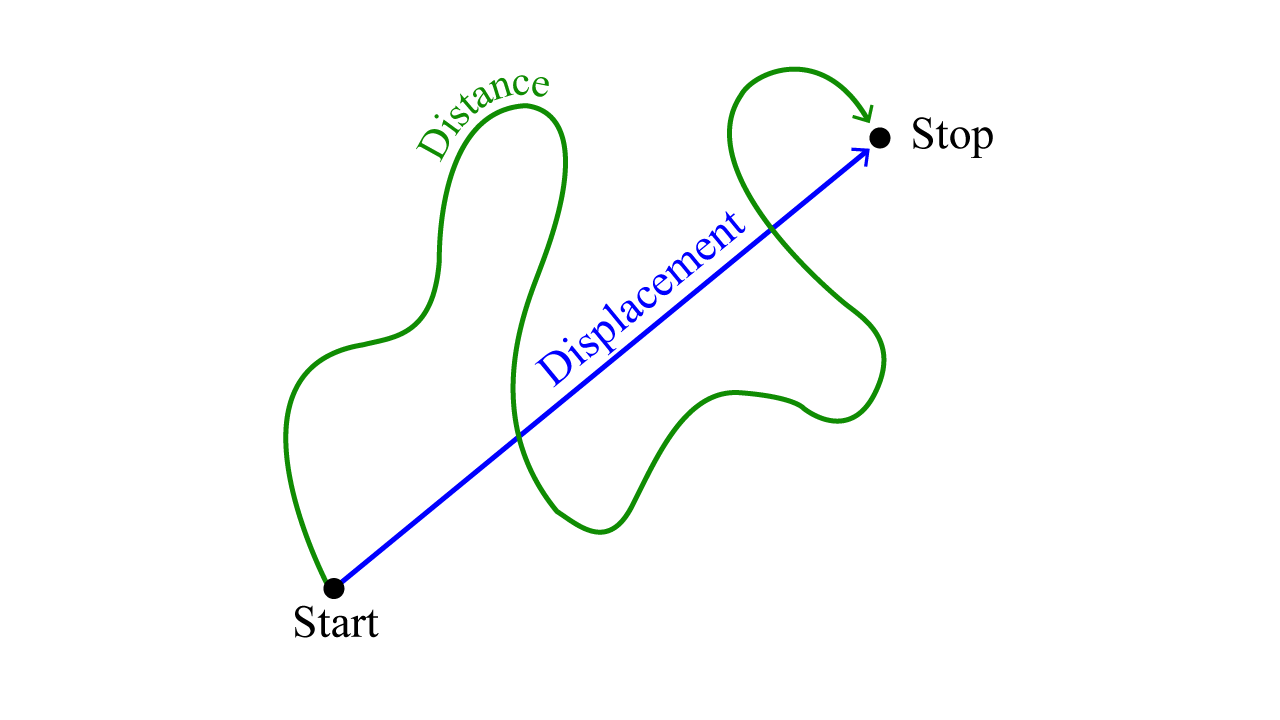
\includegraphics[scale=0.2]{images/distance-vs-displacementphoto}
	\caption{Distance vs Displacement Example}
	\label{fig:DisplacmentVsDistance}
\end{figure}
As seen above in figure \ref{fig:DisplacmentVsDistance}, a picture can help you distinguish between distance and displacement.
	
	% Average Speed and Velocity
	% Average Speed and Velocity
\section{Average Speed and Velocity}
	
% Average Speed and Velocity - Average Speed
\subsection{Average Speed}
Average speed describes how fast a particle is moving. Average speed is always a positive number. The equation for average speed is: \[s\textsubscript{ave} = \frac{d}{\Delta t}\] where: 
\begin{itemize}
	\item $s\textsubscript{ave}$ = average speed
	\item $d$ = distance
	\item $\Delta t$ = elapsed time
\end{itemize}
The SI unit of speed is the $m/s$.

% Average Speed and Velocity - Average Velocity
\subsection{Average Velocity}
Average velocity describes how fast the displacement is changing. Average velocity can either be positive or negative depending on direction. The equation for average velocity is: \[v\textsubscript{ave} = \frac{\Delta x}{\Delta t}\] where:
\begin{itemize}
	\item $v\textsubscript{ave}$ = average speed
	\item $\Delta x$ = displacement
	\item $\Delta t$ = elapsed time
\end{itemize}
The SI unit of speed is the $m/s$.
	
% Average Speed and Velocity - Instantaneous Velocity
\subsection{Instantaneous Velocity}
Instantaneous Velocity is the velocity at a single instant in time. If the velocity is uniform, or constant, the instantaneous velocity is the same as the average velocity. If the velocity is not constant, then the instantaneous velocity is not the same as the average velocity, and we must carefully distinguish between the two.
	
	% Acceleration
	% Acceleration
\section{Acceleration}
	
% Overview
\subsection{Acceleration (a)}
Any change in velocity over a period of time is called acceleration. The sign (+ or -) of acceleration indicates it's direction. Acceleration can be…
\begin{itemize}
	\item speeding up
	\item speeding down
	\item turning
\end{itemize}

% Acceleration Graphs
\subsection{Acceleration Graphs}

% Graphs
\begin{figure}[H]%
	\hfill
	\subfigure[Zero Acceleration]{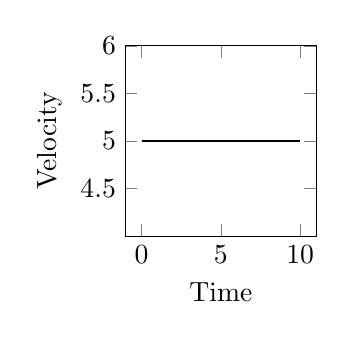
\begin{tikzpicture} \begin{axis}[xlabel = Time, ylabel = Velocity, width=4cm, height = 4cm] xmin = 0, xmax = 10, ymin = 0, ymax = 10, \addplot[domain = 0:10, smooth, thick] {5}; \end{axis} \end{tikzpicture}\label{fig:ZeroAcceleration}}
	\hfill
	\subfigure[Positive Acceleration]{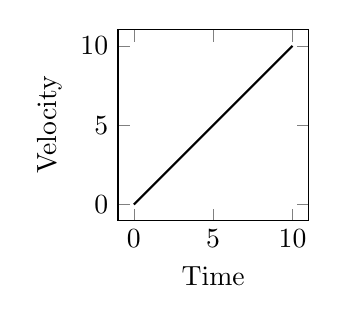
\begin{tikzpicture} \begin{axis}[xlabel = Time, ylabel = Velocity, width=4cm, height = 4cm] xmin = 0, xmax = 10, ymin = 0, ymax = 10, \addplot[domain = 0:10, smooth, thick] {x}; \end{axis} \end{tikzpicture}\label{fig:PositiveAcceleration}}
	\hfill
	\subfigure[Negative]{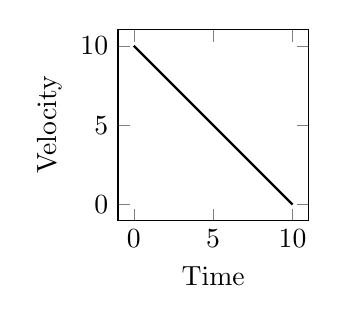
\begin{tikzpicture} \begin{axis}[xlabel = Time, ylabel = Velocity, width = 4cm, height = 4cm] xmin = 0, xmax = 10, ymin = 0, ymax = 10, \addplot[domain = 0:10, smooth, thick] {-x+10}; \end{axis} \end{tikzpicture}\label{fig:NegativeAcceleration}}
	\hfill
	\caption{Graphs of Acceleration}
	\label{fig:TypesofAccleration}
\end{figure}

As seen above in Figure \ref{fig:TypesofAccleration}, acceleration can be zero as seen in \ref{fig:ZeroAcceleration}, positive as seen in \ref{fig:PositiveAcceleration}, or negative as seen in \ref{fig:NegativeAcceleration}. 

Particles moving with no acceleration (constant velocity) have graphs of position vs time with one slope. The velocity is not changing since the slope is constant.
		
Position vs time graphs for particles moving constant acceleration look parabolic. The instantaneous slope is changing. In this graph it is increase and the particle is speeding up.
	
% Uniform (Constant) Acceleration
\subsection{Uniform (Constant) Acceleration}
In Physics 1, we will generally assume that acceleration is \textit{constant}. With this assumption we are free to use this equation: \[a=\frac{\Delta v}{\Delta t}\] 
The SI unit of acceleration is the $m/s^2$.
	
% Acceleration has a sign!
\subsection{Acceleration has a sign!}
If the sign of the velocity and the sign of the acceleration is the same, the object speeds up. If the sign of the velocity and the sign of the acceleration are different, the object slows down.
	
	% Kinematic Equations
	% Kinematic Equations
\section{Kinematic Equations Graphs}
	
% Kinematic Equations -  Position vs Time Graphs
\subsection{Position vs Time Graphs}

Particles moving with no acceleration (constant velocity) have graphs of position vs time with one slope. The velocity is not changing since the slope is constant.
		
Position vs time graphs for particles moving constant acceleration look parabolic. The instantaneous slope is changing. In this graph it is increase and the particle is speeding up.
		
\subsection{Kinematics Equations}
If you are not worried about $x$, then use this formula: \[v=v_{\circ} +at\]
If you are not worried about $v$, then use this formula: \[\Delta x = v_o*t + \frac{1}{2}at^2\]
If you are not worried about $t$, then use this formula: \[v^2=v_\circ^2+2a(\Delta x)\]
	
	% Free Fall
	% Free Fall
\section{Free Fall}
	
% Overview
\subsection{Overview}
Free fall occurs when an object falls unimpeded. Gravity accelerates the object toward the earth and the entire time it rises, and the entire tie it falls. \[a=g=9.8m/s^2\] 
	
Acceleration is always constant and toward the center of the earth and air resistance is ignored. 
	
% Symmetry in Free Fall
\subsection{Symmetry in Free Fall}
When something is throw upward and returns to the thrower, this is very symmetric. The object spends half its time traveling up and half traveling down. The velocity when it returns to the group is the opposite of the velocity it was thrown upward with. Acceleration is $9.8 m/s^2$ everywhere!
	
	% Vectors
	%Vectors
\section{Vectors}
	
% Overview
\subsection{Overview}
There are two kinds of quantities...
\begin{itemize}
	\item Scalars are the quantities that have \textbf{magnitude} only
	\begin{itemize}
		\item position
		\item speed
		\item time
		\item mass
	\end{itemize}
	
	\item Vectors are quantities that have both \textbf{magnitude} and \textbf{direction}, such as
	\begin{itemize}
		\item displacement
		\item velocity
		\item acceleration
	\end{itemize}
\end{itemize}
	
% Direction of Vectors
\subsection{Direction of Vectors}
Vector \textbf{direction} is the direction of the arrow, given by an \textbf{angle}.
	
% Magnitude of Vectors
\subsection{Magnitude of Vectors}
The best wya to determine the \textbf{magnitude} of a vector is to measure its \textbf{length}. The length of the vector \textit{proportional} to the magnitude (or size) of the quantity it represents.
	
% qual and Inverse Vectors
\subsection{Equal and Inverse Vectors}
\textbf{Equal vectors} have the \textbf{same length and direction}, and represent the same quantity (such as force or velocity).
	
\textbf{Inverse vectors} have the \textbf{same length}, but \textbf{opposite direction}.
	
% Vectors: x-component
\subsection{Vectors: x-component}
The x-component of a vector is the "shadow" it cases on the x-axis. 
\[cos \theta = \frac{\text{adjacent}}{\text{hypotenuse}}\]
	
% Vectors: y-component
\subsection{Vectors: y-component}
The y-component of a vector is the "shadow" it casts on the y-axis. 
\[sin\theta=\frac{\text{opposite}}{\text{hypotenuse}}\]
	
% Vectors: Angle
\subsection{Vectors: angle}
The angle of a vector makes with the x-axis can be determined by the components. It is calculated by the inverse tangent function
\[\theta = \tan^{-1}\frac{\text{opposite}}{\text{adjacent}}\]
	
% Vectors: magnitude
\subsection{Vectors: magnitude}
The magnitude of a vector can be determined by the components. It is calculated by using the Pythagorean Theorem. \[A^2+B^2=C^2\]
	
	% 2-D Vectors and Projectiles
	% 2-D Vectors and Projectiles
\section{2-D Vectors and Projectiles}
	
% Overview
\subsection{Overview}
2-D Dimensional Motion is motion that occurs with both x and y components. Each dimension of the motion can obey different equations of motion.
	
% How to Solve 2-D Problems
\subsection{How to Solve 2-D Problems}
\begin{enumerate}
	\item Resolve all the vectors into x and y components
	\item Work the problem as two one-dimensional problems
	\item Re-combine the results for the two components at the end of the problem. 
\end{enumerate}
	
% Projectiles Motion
\subsection{Projectile Motion}
A projectile is something is fired, throw, shot, or hurled near the earth's surface. Horizontal velocity is constant, vertical velocity is accelerated, and air resistance is ignored. 
	
% 1-D Projectiles
\subsection{1-Dimensional Projectiles}
A 1-Dimensional projectile is a projectile that movies in a vertical direction only and is subject to acceleration by gravity. Here you can only calculate vertical motion because the motion has no horizontal component.
	
% 2-D Projectiles
\subsection{2-Dimensional Projectiles}
A 2-Dimensional projectile is a projectile that moves both horizontally and vertically and is subject to acceleration by gravity in the vertical direction. Here you can calculate both vertical and horizontal motion.
	
% Horizontal Component of Velocity
\subsection{Horizontal Component of Velocity}
The horizontal component of velocity is always constant, not accelerated, and not influenced by gravity. It follows this equation: \[x=V_{ox}t\]
	
% Vertical Component of Velocity
\subsection{Vertical Component of Velocity}
The vertical component of velocity undergoes accelerated motion and is accelerated by gravity.
\[V_y=V_{oy}+gt\]
\[y=y_o+V_{oy}+\frac{1}{2}gt^2\]
\[V_y^2=V_{oy}^2+2g(y-y_o)\]
	
% Launch Angle
\subsection{Launch Angle}
Launch angle is the angle at which a projectile is launched. The launch angle determines what the trajectory for he projectile will be. Launch angles can range from $-90^\circ$ (throwing something straight down) to $+90^\circ$ (throwing something straight down) and everything in between. A zero launch angle implies a perfectly horizontal launch.
	
% General Launch Angle
\subsection{General Launch Angle}
Projectile motion is more complicated when the launch angle is not straight up or down or perfectly horizontal. You must being these types of problems by resolving the velocity vector into its components. Then use speed and the launch angle to find the horizontal and vertical velocity components. \[V_{oy}=V_o\sin\theta\]
	
Use speed and the launch angle to find both the horizontal and vertical components. 
\[V_{ox}=v_o\cos\theta\]
\[V_{oy}=v_o\sin\theta\]
	
% Projectiles launched over level ground
\subsection{Projectiles launched over level ground}
These projectiles have highly symmetric characteristics of motion. It is handy to know these characteristics, since a knowledge of the symmetry can help in working problems and predicting the motion.
	
% Trajectory of a 2-D Projectile
\subsection{Trajectory of a 2-D Projectile}
The trajectory is the path traveled by any projectile. It is plotted on an x-y graph. Mathematically, the path is defined by a parabola. For a projectiles launched over level ground, the symmetry is apparent.
	
% Range of a 2-D Projectile
\subsection{Range of a 2-D Projectile}
The range of the projectile is how far it travels horizontally.
	
% Maximum height of a 2-D Projectile
\subsection{Maximum height of a 2-D Projectile}
The maximum height of the projectile occurs when it stops moving upward. The vertical velocity component is zero at the maximum height. For a projectile launched over level ground, the maximum height occurs halfway through the flight of the projectile. 
	
% Acceleration of a Projectile
\subsection{Acceleration of a Projectile}
Acceleration points down at $9.8m/s^2$ for the entire trajectory of all projectiles. 
	
% Velocity of a Projectile
\subsection{Velocity of a Projectile}
Velocity is tangent to the path for the entire trajectory. The velocity can be resolved into components all along its path. The vertical velocity changes while the horizontal velocity remains the same. Maximum speed is attained at the beginning and again at the end of the trajectory if the projectile is launched over level ground. Launch angle is symmetric with landing angle for a projectile over level ground.
	
% Time of flight for a Projectile
\subsection{Time of flight for a Projectile}
The projectile spends half its time traveling upward and the other half traveling down.
	
% The Range Equation
\subsection{The Range Equation}
Derivation is an important part of physics. The Range equation is in your textbook but not on your formula sheet. \[R=\frac{V_o^2\sin(2\theta)}{g}\]
\begin{itemize}
	\item $R$ = Range of the projectile fired over level ground
	\item $v_o$ = initial velocity
	\item $g$ = acceleration due to gravity
	\item $\theta$ = launch angle
\end{itemize}
	
	% Newton's Laws
	% Newton's Laws
\section{Newton's Laws}
	
% Isaac Newton
\subsection{Isaac Newton}
Isaac Newton is arguably the greatest scientific genius ever. He came up with 3 Laws of Motion to explain the observations and analyses of Galileo and Johannes Kepler. He also discovered that white light was composed of many colors all mixed together. He invented new mathematical techniques such as calculus and binomial expansion theorem in his study of physics. He published his laws in 1687 in the book Mathematical Principles of Natural Philosophy.
	
% What is Force?
\subsection{What is Force?}
A force is a \textbf{push} or a \textbf{pull} on an object. Forces cause an object to \textbf{accelerate}.
	
% Newton's First Law
\subsection{Newton's First Law}
\textbf{A body in motion stays in motion at a constant velocity} and a body at rest stays at rest \textbf{unless acted upon by a net external force}. This law is commonly referred to as the \textbf{Law of Inertia}. If there is \textbf{zero net force} on a body, it cannot accelerate, and therefore must move at a constant velocity. 
	
% Mass and Inertia
\subsection{Mass and Inertia}
Chemists like to define mass as the amount of "stuff" or "matter" a substance has. Physicists define \textbf{mass} as \textbf{inertia}, which is the ability of a body to resit acceleration by a net force.
	
% Newton's Second Law
\subsection{Newton's Second Law}
A body \textbf{accelerates} when acted upon by a \textbf{net external force}. This acceleration is proportional to the net force and is in the direction which the net force acts. \[\sum F=ma\]

\begin{itemize}
	\item where $\sum F$ is the net force measured in Newtons ($N$)
	\item $m$ is mass (kg)
	\item $a$ is acceleration ($m/s^2$)
\end{itemize}
	
% Units of Force
\subsection{Units of Force}
\begin{itemize}
	\item Newton (SI System)
	\item $1N = 1kg*m/s^2$
	\item 1$N$ is the force required to accelerate a 1$kg$ mass at a rate if 1 $m/s^2$
\end{itemize}
	
% Newton's Third Law
\subsection{Newton's Third Law}
For every action there exist an \textbf{equal and opposite reaction}.
	
	% Newton's Laws in 2D
	% Newton's Laws in 2D
\section{Newton's Laws in 2D}
	
% Newton's Laws in 2D -  Newton's Third Law
\subsection{Newton's $2^{nd}$ Law in 2-D}
The situation is more complicated when forces act in more than one dimension. You must still identify all forces and draw your force diagram. You then resolve your problem into an x-problem and a y-problem.
	
% Newton's Laws in 2D -  Mass and Weight
\subsection{Mass and Weight}
Many people think \textbf{mass} and \textbf{weight} are the same thing. They are not. Mass is \textbf{inertia}, or resistance to acceleration. Weight can be defined as the \textbf{force due to gravitation attraction} \[W=mg\]
	
% Newton's Laws in 2D - Apparent Weight
\subsection{Apparent Weight}
If an object subject to gravity is not in free fall, then there must be a \textbf{reaction force} to act in opposition to gravity. We sometimes refer to this reaction force as \textbf{apparent weight}.
	
% Newton's Laws in 2D - Elevator Rides
\subsection{Elevator Rides}
When you are in an elevation, \textbf{your actual weight ($mg$) never changes}. You feel lighter or heavier during the ride because your \textbf{apparent weight} increases when you are accelerating up, decreases when you are accelerating down, and is equal to your weight when you are not accelerating at all.
	
% Newton's Laws in 2D - Normal Force
\subsection{Normal Force}
The \textbf{normal force} is a force that keeps one object from penetrating into another object. the normal force is always \textbf{perpendicular} to a surface. The normal exactly cancels out the components of all applied forces that are perpendicular to a surface. A normal force can also exist that is totally unrelated to the weight of an object.
	
% Newton's Laws in 2D - Normal Force on a flat surface
\subsection{Normal Force on a flat surface}
The normal force is equal to the weight of an object for objects resting on a horizontal surface. \[N=W=mg\]
	
% Newton's Laws in 2D - Normal Force on a ramp
\subsection{Normal Force on a ramp}
The normal force is perpendicular to angled ramps as well. It's always equal to the component of weight perpendicular to the surface. \[N=m*g*\cos\theta\]
	
	% Introduction to Friction
	% Introduction to Friction
\section{Introduction to Friction}
	
% Introduction to Friction - Overview
\subsection{Overview}
Friction is the force that opposes a sliding motion. Friction is due to microscopic irregularities in even the smoothest of surfaces. Friction is highly useful and enables us to walk and drive a car, among other things. Friction is also dissipative. That means it causes mechanical energy to be converted to head. The friction that exits between two surfaces is directly proportional to the normal force.
	
% Introduction to Friction - Static Friction
\subsection{Static Friction}
Static friction occurs between two surfaces that are not slipping relative to each other. \[f_s\leq\mu_sN\]
\begin{itemize}
	\item $f_s$ =  Static frictional force ($N$)
	\item $\mu_s$ = coefficient of static friction
	\item $N$ = normal force (N)
\end{itemize}
Static frictions between two surfaces is \textbf{zero unless there is a force} trying to make the surfaces slide on one another. Static friction can \textbf{increase} as the force trying to push an object \textbf{until it reaches its maximum allowed value as defined by $\mu_s$} Once the maximum value of static friction has been exceeded by an applied force, the surfaces begin to slide and the friction is no longer static friction.
	
% Introduction to Friction - Kinetic Friction
\subsection{Kinetic Friction}
Kinetic friction \textbf{occurs between surfaces that are slipping past each other}. \[f_k=\mu_kN\]
\begin{itemize}
	\item $f_k$ = kinetic frictional force ($N$)
	\item $\mu_k$ = coefficient of kinetic friction
	\item $N$ = normal force ($N$)
\end{itemize}
Kinetic friction (sliding friction) is \textbf{generally less than static friction} (motionless friction) for most surfaces.
	
	% Introduction to Work
	% Kinematics
\section{Introduction to Work}

% Overview
\subsection{Overview}
Work tells us how much a force or combination of forces changes the energy of a system. Work is the bridge factor between force (a vector) and energy (a scalar).
\[W=F(\Delta x)\cos\theta\]
Where:
\begin{itemize}
	\item $F$ = Force ($N$)
	\item $\Delta x$ = Displacement ($m$)
	\item $\theta$ = Angle between force and displacement
\end{itemize}

Forces and direction of motion also both matter in defining work. There is no work done by a force if it causes no displacement. Forces can do positive, negative, or zero work. 

% Units of Work
\subsection{Units of Work}
\begin{itemize}
	\item SI System: Joule ($Nm$)
	\item British System: foot-pound
	\item cgs System: erg (dyne-cm)
	\item Atomic Level: electron-Volt (eV)
\end{itemize}

% Work and Energy
\subsection{Work and Energy}
Work changes mechanical energy! If an applied force does positive work on a system, it tries to increase mechanical energy. If an applied force does negative work, it tries to decrease mechanical energy. The two forms of mechanical energy are called potential and kinetic energy.

% Kinetic Energy
\subsection{Kinetic Energy}
Kinetic Energy is energy due to motion. \[K=\frac{1}{2}mv^2\] Where:
\begin{itemize}
	\item $K$ = Kinetic Energy
	\item $m$ = mass in $kg$
	\item $v$ = speed in $m/s$
\end{itemize}

% The Work-Energy Theorem
\subsection{The Work-Energy Theorem}
The Work-Energy Theorem states that the net work due to all forces equals the change in the kinetic energy of a system. \[W\textsubscript{net}=\Delta K\] Where:
\begin{itemize}
	\item $W\textsubscript{net}$ = work due to all forces acting on an object
	\item $\Delta K$ = change in kinetic energy ($K_f-K_i$)
\end{itemize}

% Springs
\subsection{Springs}
When a spring is stretched or compressed from it equilibrium position, it does \textbf{negative work}, since the spring pulls opposite the direction of motion. \[W_s=-\frac{1}{2}kx^2\] Where:
\begin{itemize}
	\item $W_s$ = work done by spring $J$
	\item $k$ = force constant of spring ($N/m$)
	\item $x$ = displacement from equilibrium ($m$)
\end{itemize}
The force doing the stretching does \textbf{positive work} equal to the magnitude of the work done by the spring. \[W\textsubscript{applied}=-\frac{1}{2}kx^2\]

% Spring Tension
\subsection{Tension}
Tension is a \textbf{pulling force} that arises when a \textbf{rope, string, or other long thin material resists being pulled apart} without stretching significantly. Tension always pulls away from a body attached to a rope or string and toward the center of the rope or string. 
	
% Springs (Hooke's Law)
\subsection{Springs (Hooke's Law)}
The magnitude of the force exerted by a spring is proportional to the amount it is stretched. \[F=-kx\] 
\begin{itemize}
	\item $F$ = force exerted by the spring ($N$)
	\item $k$ = force constant of the Spring ($N/m$ or $N/cm$)
	\item $x$ = displacement from equilibrium position ($m$ or $cm$)
\end{itemize}

% Power
\subsection{Power}
Power is the rate of which work is done. \[P=\frac{W}{\Delta t}=\frac{F\Delta x}{\Delta t} = Fv\] Where:
\begin{itemize}
	\item $W$ = work in Joules
	\item $\Delta t$ = elapses time in seconds.
\end{itemize}

% Unit of Power
\subsection{Unit of Power}
The SI unit for Power is the Watt It is named after the Scottish engineer James Watt (1776-1819) who perfected the steam engine. \[1 Watt = 1 Joule/s\] The kilowatt-hour is a commonly used unit by electrical power companies. Power companies charge you by the kilowatt-hour ($kWh$) but this is not power, it is really energy consumed. \[1kW = 1000W=1000J/s*3600s=3.6*10^6J\]

% Forces Types
\subsection{Forces Types}
Forces acting on a system can be divided into two types according to how they affect potential energy. \\\textbf{Conservative forces} can be related to potential energy changes. \\\textbf{Non-conservative forces} cannot be related to potential energy changes.

% Conservative Forces
\subsection{Conservative Forces}
In conservative forces:
\begin{itemize}
	\item Work is \textbf{path independent}. Work can be calculated from the starting and ending points only. The actual path is ignored in calculations.
	\item \textbf{Work along a closed path is zero}. If the starting and ending points are the same, no work is done by the force.
	\item \textbf{Work changes potential energy}.
	\item \textbf{Conservation of mechanical energy holds!}
\end{itemize}

% Non-Conservative Forces
\subsection{Non-Conservative Forces}
In non-conservative forces:
\begin{itemize}
	\item Work is \textbf{path dependent}. Knowing the starting and ending points is not sufficient to calculate the work.
	\item \textbf{Work along a closed path is NOT zero}.
	\item \textbf{Work changes mechanical energy}.
	\item \textbf{Conservation of mechanical energy does not hold!}
\end{itemize}

% Potential Energy
\subsection{Potential Energy}
Potential Energy is the energy of position or configuration. It is also know as "stored" energy. 
\begin{itemize}
	\item For gravity: $U_g=mgh$
	\begin{itemize}
		\item $m$ = mass
		\item $g$ = acceleration due to gravity
		\item $h$ = height above the "zero" point
	\end{itemize}
	
	\item For springs: $U_s=\frac{1}{2}kx^2$
	\begin{itemize}
		\item $k$ = spring force constant
		\item $x$ = displacement from equilibrium position
	\end{itemize}
\end{itemize}

% Conservative forces and Potential energy
\subsection{Conservative forces and Potential energy}
\[W_c=-\Delta U\] If a conservative force does positive work on a system, potential energy is lost. If a conservative force does negative work , potential energy is gained.
\begin{itemize}
	\item For Gravity: $-W_g=-\Delta U_g=-({mgh}_f-{mgh}_i)$
	\item For Springs: $-W_s=-\Delta U=-(\frac{1}{2}kx_f^2-\frac{1}{2}kx_i^2)$
\end{itemize}
	
	% Conservation of Energy
	% Conservation of Energy
\section{Conservation of Energy}

% Law of Conservation of Energy
\subsection{Law of Conservation of Energy}
In any isolated system, the total energy remains constant. Energy can neither be created nor destroyed, but can only be transformed from one type of energy to another. 

% Conservation of Mechanical Energy
\subsection{Law of Conservation of Mechanical Energy}
\begin{itemize}
	\item E = K+U = Constant
	\begin{itemize}
		\item K = Kinetic Energy ($\frac{1}{2}mv^2$)
		\item U = Potential Energy (gravity or spring)
	\end{itemize}
	
	\item $\Delta$E = $\Delta$U + $\Delta$K = 0
		\begin{itemize}
		\item $\Delta$K = Change in kinetic energy
		\item $\Delta$U = Change in gravitational or spring potential energy
	\end{itemize}
\end{itemize}

% Pendulums and Energy Conservation
\subsection{Pendulums and Energy Conservation}
Energy goes back and forth between K and U. At the highest point, all energy is U. As it drops, U goes to K. At the bottom, energy is all K.

% Springs and Energy Conservation
\subsection{Springs and Energy Conservation}
Transforms energy back and forth between K and U. When fully stretched or extended, all energy is U. When passing through equilibrium, all its energy is K. At other points in its cycle, the energy is a mixture of U and K.

% Law of Conservation of Energy Formula
\subsection{Law of Conservation of Energy Formula}
\begin{itemize}
	\item E = U + k+ E$\textsubscript{initial}$ = Constant
	\item $\Delta$U + $\Delta$K + $\Delta$E$\textsubscript{initial}$ = 0
	\item E$\textsubscript{inital}$ is thermal energy.
	\item Mechanical energy may be converted to and from heat.
\end{itemize}

% Work done by non-conservative forces
\subsection{Work done by non-conservative forces}
\begin{itemize}
	\item $W\textsubscript{net}=W_c+W_{nc}$
	\begin{itemize}
		\item Net work is done by conservative and non-conservative forces
		\item $W_c = -\Delta U$
		\item $W\textsubscript{net}=\Delta K$
		\item $\Delta K = -\Delta U + W_{nc}$
	\end{itemize}
	\item $W_{nc}=\Delta U + \Delta K = \Delta E$
	\item Non-conservative forces change mechanical energy. If non-conservative work is negative, as it often is, the mechanical energy of the system will drop.
\end{itemize}
	
	% Momentum
	% Momentum
\section{Momentum}

% Overview
\subsection{Overview}
\textbf{Momentum is a measure of how hard it is to stop or turn a moving object.} Momentum is related to both mass and velocity. Momentum is possessed by all moving objects.

% Calculating Momentum
\subsection{Calculating Momentum}
\begin{itemize}
	\item For one particle: $p=mv$ 
	\item For a system of multiple particles: $P=\sum P_i=\sum m_iv_i$\
	\item Momentum is a vector with the same direction as the velocity vector
	\item The unit of Momentum is $kg*m/s$ or $Ns$
\end{itemize}

% Change in momentum
\subsection{Change in Momentum}
Like any change, change is momentum is calculated by looking at final and initial momentum. \[\Delta p = p_f-p_i\]
\begin{itemize}
	\item $\Delta p$ = Change in momentum
	\item $p_f$ = Final momentum
	\item $p_i$ = initial momentum
\end{itemize}

% Impulse
\subsection{Impulse}
\textbf{Impulse} is the \textbf{product of} an external \textbf{force and time}, which results in a \textbf{change in momentum} of a particle or system. \[J=F*t\] \[J=\Delta P\] Impulsive forces are usually \textbf{high magnitude} and \textbf{short duration}. 

% Law of Conservation of Momentum
\subsection{Law of Conservation of Momentum}
If the resultant external force on a system is zero, then the vector sum of the momentums of the objects will remain constant. \[\sum P\textsubscript{before}=\sum P\textsubscript{after}\]

% External versus Internal Forces
\subsection{External versus internal forces}
\textbf{External forces} are forces coming from outside the system of particles whose momentum is being considered. \textbf{Internal forces} are forces arising from interaction of particles within a system. External forces change the momentum of the system while internal forces do not.

% Explosions
\subsection{Explosions}
When an object separates suddenly, as in an explosion, all forces are internal. Momentum is therefore conserved in an explosion. There is also an increase in kinetic energy in an explosion., This comes from a potential energy decrease due to chemical combustion.

% Recoil
\subsection{Recoil}
Guns and cannons \textbf{"recoil"} when fired. \textbf{This means the gun or cannon must move backwards as it propels the projectile forward.} The recoil is the result of action0reaction force pairs, and is entirely due to internal forces. As the gasses from the gunpowder explosion expand, they push the projectile forwards and the gun or cannon backwards. 
	
	% Collisions
	% Collisions
\section{Collisions}

% Overview
\subsection{Overview}
When two moving objects make contact with each other, they undergo a \textbf{collision}. Conservation of momentum is used to analyze all collisions. Newton's Third law is also useful. It tells us that a force exerted by body A on body B in a collision is equal and opposite to the force exerted on body B by body A. During a collision, external forces are ignored. The time frame of the collision is also very short and the forces are impulsive forces.

% Collision Types
\subsection{Collision Types}
\begin{itemize}
	\item \textbf{Elastic Collisions} - No deformation occurs and no kinetic energy is lost
	\item \textbf{Inelastic Collisions} - Deformation occurs and kinetic energy is lost
	\item \textbf{Perfectly Inelastic Collisions} - Objects stick together and become one object. Deformation also occurs and kinetic energy is lost
\end{itemize}

% (Perfectly) Inelastic Collisions
\subsection{(Perfectly) Inelastic Collisions}
This is the simplest type of collision. After the collision, there is only one velocity, since there is only one object. Kinetic energy is also lost. Explosions are the reverse of perfectly inelastic collisions in which kinetic energy is gained. 

% Elastic Collisions
\subsection{Elastic Collisions}
After the collision, there are still two objects but with two separate velocities. Kinetic energy remains constant before and after the collision and therefore, two basic equations must hold true for all elastic collision: \[\sum p_b =\sum p_a\] \[\sum K_b =\sum K_a\]

% 2D Collisions
\subsection{2D Collisions}
Momentum in the x-direction is conserved:
\[\sum P_x\mbox{ (before) }= \sum P_x\mbox{ (after) }\]

Momentum in the y-direction is conserved:
\[\sum P_y\mbox{ (before) }= \sum P_y\mbox{ (after) }\] 

You must treat x and y coordinates independently. You ignore x when calculating y and ignore y when calculating x.
	
	% The Universal Law of Gravity
	% The Universal Law of Gravity
\section{The Universal Law of Gravity}

% Overview
\subsection{Overview}
The Universal Law of Gravity tells us that the force of gravity objects exert on each other depends on their masses and the distance they are separated from each other. You used the formula $F_g=mg$ to approximate the force of gravity on an object near the earth's surface. This formula wont work for planets, space travel or for objects that are far from earth.

% The Force of Gravity
\subsection{The Force of Gravity}
The Universal Law of gravity \textbf{always} works, whereas $F_g=mg$ only works sometimes. \[F_g=\frac{Gm_1m_2}{r^2}\]
\begin{itemize}
	\item $F_g$ = Force due to gravity ($N$)
	\item $G$ = Universal gravitational constant $6.67*10^-11\frac{Nm^2}{kg^2}$
	\item $m_1$ and $m_2$ = the two masses ($kg$)
	\item $r$ = the distance between the cents of the masses ($m$)
\end{itemize}

% Acceleration due to Gravity
\subsection{Acceleration due to Gravity}
$g=9.8m/s^2$ works fine when we are near the surface of the earth, For space travel, we need a different formula. \[g=\frac{GM}{r^2}\] 

This formula lets you calculate $g$ anywhere if you know the distance a body is from the center of a planet and you can use it to calculate the acceleration to gravity anywhere.
	
	% Uniform Circular Motion
	% Uniform Circular Motion
\section{Uniform Circular Motion}

% Overview
\subsection{Overview}
Uniform circular motion is the motion of an object traveling at a constant speed on a circular path. \[\mbox{The distance the object travels: } d=2\pi r\] \[\mbox{The speed of the object: } v=\frac{2\pi r}{T}\]

In uniform circular motion, the speed is constant but the velocity is not. The object is constantly changing directions so it is constantly acceleration. The acceleration is called centripetal acceleration. 

% Centripetal Acceleration
\subsection{Centripetal Acceleration}
Centripetal acceleration is always directed toward the center of the circle. \[a_c=\frac{v^2}{r}\]

% Centripetal Force
\subsection{Centripetal Force}
Centripetal force is always directed toward the center of the circle. This force is not a unique force but instead it must be provided by some other force. \[\sum F = \frac{mv^2}{r}\]

% Centrifugal Force
\subsection{Centrifugal Force}
This is the forbidden force. It is not a real force but instead it is the way we fell about centripetal force.
	
	% Rotational Kinematics
	% Rotational Kinematics
\section{Rotational Kinematics}

% Overview
\subsection{Overview}
In the simplest kind of rotation, points on a rigid object move on circular paths around the \textbf{axis of rotation}. The angle though which the object rotates is called the \textbf{angular displacement}. \[\Delta \theta = \theta - \theta_o\]

% Rotational Motion and Angular Displacement
\subsection{Rotational Motion and Angular Displacement}
When a rigid body rotates around a fixed axis, the angular displacement is the angle swept out by a line passing through any point on the body and intersecting the axis of rotation perpendicularly. By convention, the angular displacement is positive if it is counter clockwise and negative if it is clockwise. The SI Unit of Angular Displacement is the radian (rad).
\[\theta = \frac{2\pi r}{r}=2\pi \text{rad}\]

\[\theta = \frac{\text{Arc Length}}{\text{Radius}}=\frac{s}{r}\]

% Angular Velocity and Angular Acceleration
\subsection{Angular Velocity and Angular Acceleration}
Changing angular velocity means that an \textbf{angular acceleration} is occurring. 
\[\overline{\omega} =\frac{\theta-\theta_o}{t-t_o}=\frac{\Delta \theta}{\Delta t}\]

\[\overline{\alpha}=\frac{\omega-\omega_o}{t-t_o}=\frac{\Delta \omega}{\Delta t}\]

% Instantaneous Angular Velocity
\subsection{Instantaneous Angular Velocity}
\[\omega = \lim_{\Delta t\to 0}\overline{\omega}=\lim_{\Delta t\to 0}\frac{\Delta \theta}{\Delta t}\]

% The Equations of Rotational Kinematics
\subsection{The Equations of Rotational Kinematics}
\[\omega=\omega_o+\alpha t\]
\[\theta=\frac{1}{2}(\omega_o+\omega)t\]
\[\omega^2=\omega^2_o+2\alpha t^2\]
\[\omega = \sqrt{\omega^2_o + 2 \alpha\Delta\theta}\]
\[\Delta \theta=\omega_o t+\frac{1}{2}\alpha t^2\]
Where: \begin{itemize}
	\item $\theta$ = Displacement
	\item $\omega_o$ = Initial Velocity
	\item $\omega$ = Final Velocity
	\item $\alpha$ = Acceleration
	\item $t$ = Time
\end{itemize}

% Angular Variables and Tangential Variables
\subsection{Angular Variables and Tangential Variables}
\[\overrightarrow{V_T} = \text{tangential velocity}\]
\[V_T = \text{tangential speed}\]

\[v_T=\frac{s}{t}=\frac{r\theta}{t}=r\left(\frac{\theta}{t}\right)=r\omega\]
\[v_T=r\omega\]

\[a_T=\frac{v_t-v_{To}}{t}=\frac{(r\omega)-(r\omega_o)}{t}=r\frac{\omega-\omega_o}{t}=r\alpha\]
\[a_T=r\alpha\]

% Centripetal Acceleration and Tangential Acceleration
\subsection{Centripetal Acceleration and Tangential Acceleration}
\[a_c=\frac{v^2_T}{r}=\frac{(r\omega)^2}{r}=r\omega^2\]

% Rolling Motion
\subsection{Rolling Motion}
The tangential speed of a point on the outer edge of a tire is equal to the speed of a car over the ground. 
\[v=r\omega\]
\[a=r\alpha\]




















	
\end{document}